\documentclass[]{tukediphc}
%% -----------------------------------------------------------------
%% tento subor ma kodovanie utf-8
%%
%% na kompilaciu pouzivajte format pdfcslatex 
%%
%% vytvorene distribuciou texlive 2009-7, OS GNU/Linux
%% vytvorene distribuciou TeXLive 2010, OS Win XP
%% februar 2013
%% -----------------------------------------------------------------
\usepackage[utf8]{inputenc}
%\usepackage[T1]{fontenc}
\usepackage{lmodern,textcase}
\usepackage[slovak]{babel}\renewcommand{\figurename}{Obr\'azok}
\def\refname{Zoznam pou\v{z}itej literat\'ury}
\usepackage{latexsym}
\usepackage{dcolumn} % zarovnanie cisiel v tabulke podla des. ciarky
\usepackage{hhline}
\usepackage{subfig}
\usepackage{amsmath}
\usepackage{nicefrac} % pekne zlomky
\usepackage{upgreek} % napr. $\upmu\mathrm{m}$ pre mikrometer ...
\usepackage[final]{showkeys}%color%notref%notcite%final
\usepackage[slovak,noprefix]{nomencl}
\makeglossary % prikaz na vytvorenie suboru .glo
\usepackage{parskip}% 'zhusti' polozky obsahu
%%
%\usepackage[dvips]{graphicx}
%\DeclareGraphicsExtensions{.eps}
\usepackage[pdftex]{graphicx}
\DeclareGraphicsExtensions{.pdf,.png,.jpg,.mps}
\graphicspath{{figures/}} % priecinok na obrazky
%%
%% Cislovane citovanie
%\usepackage[numbers]{natbib}
%%
%% Citovanie podľa mena autora a roku
\usepackage{natbib} \citestyle{chicago}
% -----------------------------------------------------------------
%% tlač !!!
\usepackage[pdftex,unicode=true,bookmarksnumbered=true,
bookmarksopen=true,pdfmenubar=true,pdfview=Fit,linktocpage=true,
pageanchor=true,bookmarkstype=toc,pdfpagemode=UseOutlines,
pdfstartpage=1]{hyperref}
\hypersetup{%
baseurl={http://www.tuke.sk/sevcovic},
pdfcreator={pdfcsLaTeX},
pdfkeywords={Riadenie procesov, Oceliarstvo, Vizualizácia, Virtuálna realita, Matematické modelovanie},
pdftitle={Písomná príprava k predmetu Matematické metódy identifikácie, modelovania a simulácie},
pdfauthor={Michal Takáč},
pdfsubject={Dizertačná skúška}
} 
%% nehodiace zakomentujte !
%\dippraca{Písomná príprava k predmetu Riadenie procesov}
%\bakpraca{Príprava na dizertačnú skúšku}
%%
\nazov{Písomná príprava k predmetu Matematické metódy identifikácie, modelovania a simulácie}
%% ked praca nema 'podnazov' zakomentujte nasledujuci riadok
%% alebo polozku nechajte prazdnu
\podnazov{}
\autor{Ing.~Michal Takáč}
\veduciprace{prof.~RNDr.~Igor~Podlubný, DrSc.}
\univerzita{Technická univerzita v~Košiciach}
\fakulta{Fakulta baníctva, ekológie, riadenia a geotechnológií}
\skratkafakulty{FBERG}
\katedra{Ústav riadenia a informatizácie výrobných procesov}
\skratkakatedry{URIVP}
\odbor{Riadenie procesov}
\specializacia{Kybernetika}
\abstrakt{Abstrakt je povinnou súčasťou každej práce. Je výstižnou
charakteristikou obsahu dokumentu. Nevyjadruje hodnotiace stanovisko
autora. Má byť\/ taký informatívny, ako to povoľuje podstata práce.
Text abstraktu sa píše ako jeden odstavec. Abstrakt neobsahuje odkazy
na samotný text práce. Mal by mať\/ rozsah 250 až 500 slov. Pri
štylizácii sa používajú celé vety, slovesá v činnom rode a tretej
osobe. Používa sa odborná terminológia, menej zvyčajné termíny,
skratky a~symboly sa pri prvom výskyte v texte definujú.}
\klucoveslova{Riadenie procesov, Oceliarstvo, Vizualizácia, Virtuálna realita, Matematické modelovanie}
\datumodovzdania{30. 5. 2020}
\mesto{Košice}

\begin{document}
\renewcommand\theHfigure{\theHsection.\arabic{figure}}
\renewcommand\theHtable{\theHsection.\arabic{table}}
\bibliographystyle{dcu}

\prvastrana


\thispagestyle{empty}
\tableofcontents
\newpage
%
%\thispagestyle{empty}
%%\addcontentsline{toc}{section}{\numberline{}Zoznam obrázkov}
%\listoffigures
%\newpage
%
%\thispagestyle{empty}
%%\addcontentsline{toc}{section}{\numberline{}Zoznam tabuliek}
%\listoftables
%\newpage

%%%%%%%%%%%%%%%%%%%%%%%%%%%%%%%%%

\setcounter{page}{1}
\setcounter{equation}{0}
\setcounter{figure}{0}
\setcounter{table}{0}

\section{Úvod}

V kyslíkovom konvertore prebieha množstvo chemických reakcií a fyzikálnych javov, medzi ktorými sa nájdu aj také, ktorým úplne nerozumieme z dôvodu ich komplexnosti. Podstatou výroby ocele v takomto konvertore je oxidácia prvkov z kovonosnej vsádzky s kyslíkom fúkaným do konvertora. Oxidy týchto prvkov prechádzajú do trosky alebo odchádzajú vo forme konvertorového plynu. V kombinácii s fúkaním kyslíka prebieha proces miešania, aby sa podporila defosforizácia, dekarbonizácia, zahrievanie roztavenej ocele a homogenizácia zloženia a teploty ocele.

Rýchla dynamika procesu výroby ocele kyslíkovým konvertorom sťažuje dosiahnutie stabilných podmienok pre fúkanie kyslíka a súčasne dosiahnutie požadovaného zloženia ocele a teploty v koncovom bode tavenia. Nelineárna povaha chemických a termodynamických procesov pri výrobe ocele v LD konvertore tiež vzbudila záujem o vývoj nových matematických modelov založených na neceločíselnom diferenciálnom počte.

Matematický model predstavuje súbor funkčných vzťahov, ktoré transformujú vstupné hodnoty na výsledky, ktorými je možné vyjadriť podstatu modelovaného deja. Modelovanie je pravdepodobne najdôležitejšia časť procesu simulácie. Jej cieľom je čo najpresnejšie zachytiť správanie sa reálneho systému. Zahŕňa identifikáciu problému a očakávaný cieľ riešenia problému, zber reálnych dát alebo generácia náhodných dát, vytvorenie modelu, jeho úprava, prispôsobovanie a jeho overenie porovnaním výstupných dát zo simulácie s reálnymi dátami z reálneho systému.

\section{Počítačom podporované matematické modelovanie}

Počítačom podporované inžinierstvo (CAE - Computer Aided Engineering) je použitie počítačového softvéru na simuláciu výkonu s cieľom vylepšiť návrhy výrobkov alebo pomôcť pri riešení technických problémov pre celý rad priemyselných odvetví. To zahŕňa simuláciu, validáciu a optimalizáciu produktov, procesov a výrobných nástrojov.

Typický proces CAE pozostáva z krokov predbežného spracovania, riešenia a následného spracovania. Vo fáze predspracovania inžinieri modelujú geometriu (alebo reprezentáciu systému) a fyzikálne vlastnosti návrhu, ako aj prostredie vo forme aplikovaného zaťaženia alebo obmedzení. Ďalej je model vyriešený pomocou vhodnej matematickej formulácie základnej fyziky. Vo fáze po spracovaní sa výsledky predložia technikovi na preskúmanie.

V metalurgii pri výrobe ocele je veľmi dôležité simulovať lineárne a nelineárne procesy, s ktorými sa pri výrobe ocele stretávame pri tvorbe matematických modelov. Motivácia na používanie počítačových simulácií na skúmanie metalurgických procesov je dvojaká. Po prvé, umožňuje testovať zmeny dizajnu pred vytvorením prototypu, čo samozrejme vedie k nižším celkovým nákladom na návrh. Po druhé, umožňuje skúmať javy, ktoré sa nedajú ľahko merať alebo pozorovať v procese. Dokonca aj zdanlivo jednoduchá operácia, ako napríklad nepretržité meranie teploty počas procesu oduhličovania, je zložitá z dôvodu veľmi vysokých teplôt v procese a všeobecne drsných podmienok prevládajúcich v oceliarňach \citep{Ersson2018}.

Problémy s modernou mechanikou tekutín by nebolo možné vyriešiť bez použitia počítačovej dynamiky tekutín (CFD - Computational Fluid Dynamics). CFD je vetva CAE, ktorá sa zaoberá simuláciou pohybu tekutín a prenosom tepla pomocou numerických prístupov, pretože rozsah analytických riešení základných rovníc mechaniky tekutín je veľmi obmedzený a hlavne veľmi obtiažny. V prípade zložitejšej geometrie to znamená, že je výhodnejšie zvoliť numerickú metódu. 

\section{Počítačová dynamika tekutín (CFD)}

Počítačová dynamika tekutín (CFD) je využívaná v oboroch fyziky akými sú aerodynamika, termodynamika alebo hydrodynamika. Na makroskopickej škále je založená na numerickom riešení modelovanej sústavy parciálnych diferenciálnych rovníc, ktoré popisujú určité formy pohybu (teploty, hmotnosti, hybnosti) a ktoré vyjadrujú zákon zachovania hmotnosti (rovnica kontinuity), zákon zachovania hybnosti (Navier-Stokesove rovnice) a zákon zachovania energie (rovnice prenosu tepla konvekciou, kondukciou alebo radiáciou). Z dôvodu ich zložitosti sa miesto analytických prístupov využívajú numerické metódy, akými sú napríklad metóda konečných elementov (FEM - Finite Element Method), metóda konečných objemov (FVM - Finite Volume Method), metóda konečných rozdielov (FDM - Finite Difference Method).

Pri skúmaní dynamických javov tekutín je cieľom CFD analýzy vytvoriť čo najpresnejší obraz o týchto javoch a procesoch, ktoré vznikajú a prebiehajú pri pohybe plynných a kvapalných látok v okolí alebo vo vnútri objektov v pevnom skupenstve. Presnosť CFD simulácií ale nie je zaručená a tak treba stále počítať s tým, že nám vedia poskytnúť iba približné informácie o tom, ako sa bude simulovaná súčiastka alebo proces správať v reálnom svete. 

Pohyb tekutín súvisí s~rôznymi problémami, ktoré popisujú fyzikálne modely, ako napríklad laminárne a~turbulentné prúdenie, stlačiteľné a nestlačiteľné prúdenie, prenos a distribúcia tepla, prenos chemických prímesí vrátane chemických reakcií, viacfázové prúdenie, prúdenie poréznym prostredím, vznik bublín alebo horenie.

Metódami numerickej matematiky, formuláciou okrajových a počiatočných podmienok sa z úlohy mechaniky tekutín formuluje matematický problém. Z formulácie určujúcich rovníc (fyzikálny model), ktoré sa spravidla nedajú riešiť analyticky, sa diskretizáciou získajú algebraické rovnice (matematický model). Okrajové podmienky určujú, ako systém (napríklad štruktúra alebo tekutina) interaguje s prostredím. Fixácie, zaťaženia, tlaky, prietok alebo rýchlosť tekutiny sú príklady okrajových podmienok. Počiatočné podmienky definujú počiatočné hodnoty pre každé pole riešenia a sú vyjadrené fyzikálnymi veličinami. V priebehu riešenia sa menia každou iteráciou. Majú vplyv na čas dosiahnutia konvergencie riešenia úlohy, tj. dobu výpočtu. Samotná úloha je taktiež určená geometrickou štruktúrou (geometrický model).

V prvých štádiách nastavenia simulácie je potrebné definovať a vymedziť skúmanú oblasť v 2D alebo 3D, ktorá zahŕňa predmet modelovania a jeho najbližšie okolie. Táto oblasť sa pokryje sieťou (softvér to vie spraviť automaticky), to znamená, že sa rozdelí do určitého počtu 2D alebo 3D buniek (elementov). Počet buniek môže byť na rôznych miestach variabilný - to, koľkými bunkami je tvorená časť priestoru udáva, ako presná bude simulácia v danej oblasti. Detailnosť siete určuje aj čas výpočtov (čím detailnejšia, tým je simulácia zdĺhavejšia). Fyzikálne veličiny sú počítané pre geometrický stred každej bunky, hodnoty v ostatných miestach buniek sú interpolované alebo extrapolované.

\subsection{CFD v metalurgii}

Od počiatku priekopníckej práce v oblasti metalurgie, ktorú uskutočnili \cite{dilawari1977}, bolo vyvinutých veľa modelov, konkrétne pre kyslíkové konvertory to boli modely procesu zmiešavania, napenenia trosky, interakcií plyn-kvapalina, viacfázových tokov, ako aj aspektov prenosu tepla a hmoty \citep{chattopadhyay2010}. Náklady na vykonávanie počítačových simulácií sa za posledných niekoľko desaťročí znížili, zatiaľ čo dostupný výpočtový výkon sa zvýšil. Súčasne dostupné procesory sú štandardne viacjadrové, vďaka čomu je možné vykonávať viacero výpočtov súbežne. Pre zložité výpočty sa začali využívať grafické výpočtové jednotky (GPU) kvôli možnej paralelizácii výpočtových algoritmov. Štúdia z posledných dvoch desaťročí \citep{Ersson2018} využívania CFD simulácií v metalurgii odhaľuje obrovské zlepšenie týkajúce sa typu javov, ktoré je možné vďaka  nim preskúmať a tento trend bude  aj naďalej pokračovať. Ich použitie v oceliarskom priemysle však ešte stále nie je tak intenzívne ako v leteckom a automobilovom priemysle, v ktorých je vývoj nových dizajnov kľúčový. Hlavný rozdiel medzi leteckým a metalurgickým priemyslom spočíva v tom, že metalurgia sa takmer vždy zaoberá viacfázovými systémami pri zvýšených teplotách a že motiváciou modelovania je najmä optimalizácia procesov. S pokračujúcim vývojom vo viacfázových modeloch, ako aj pri reakčnom modelovaní toku, je užitočnosť CFD v metalurgii jasná.

\begin{figure}[!ht]
	\centering
	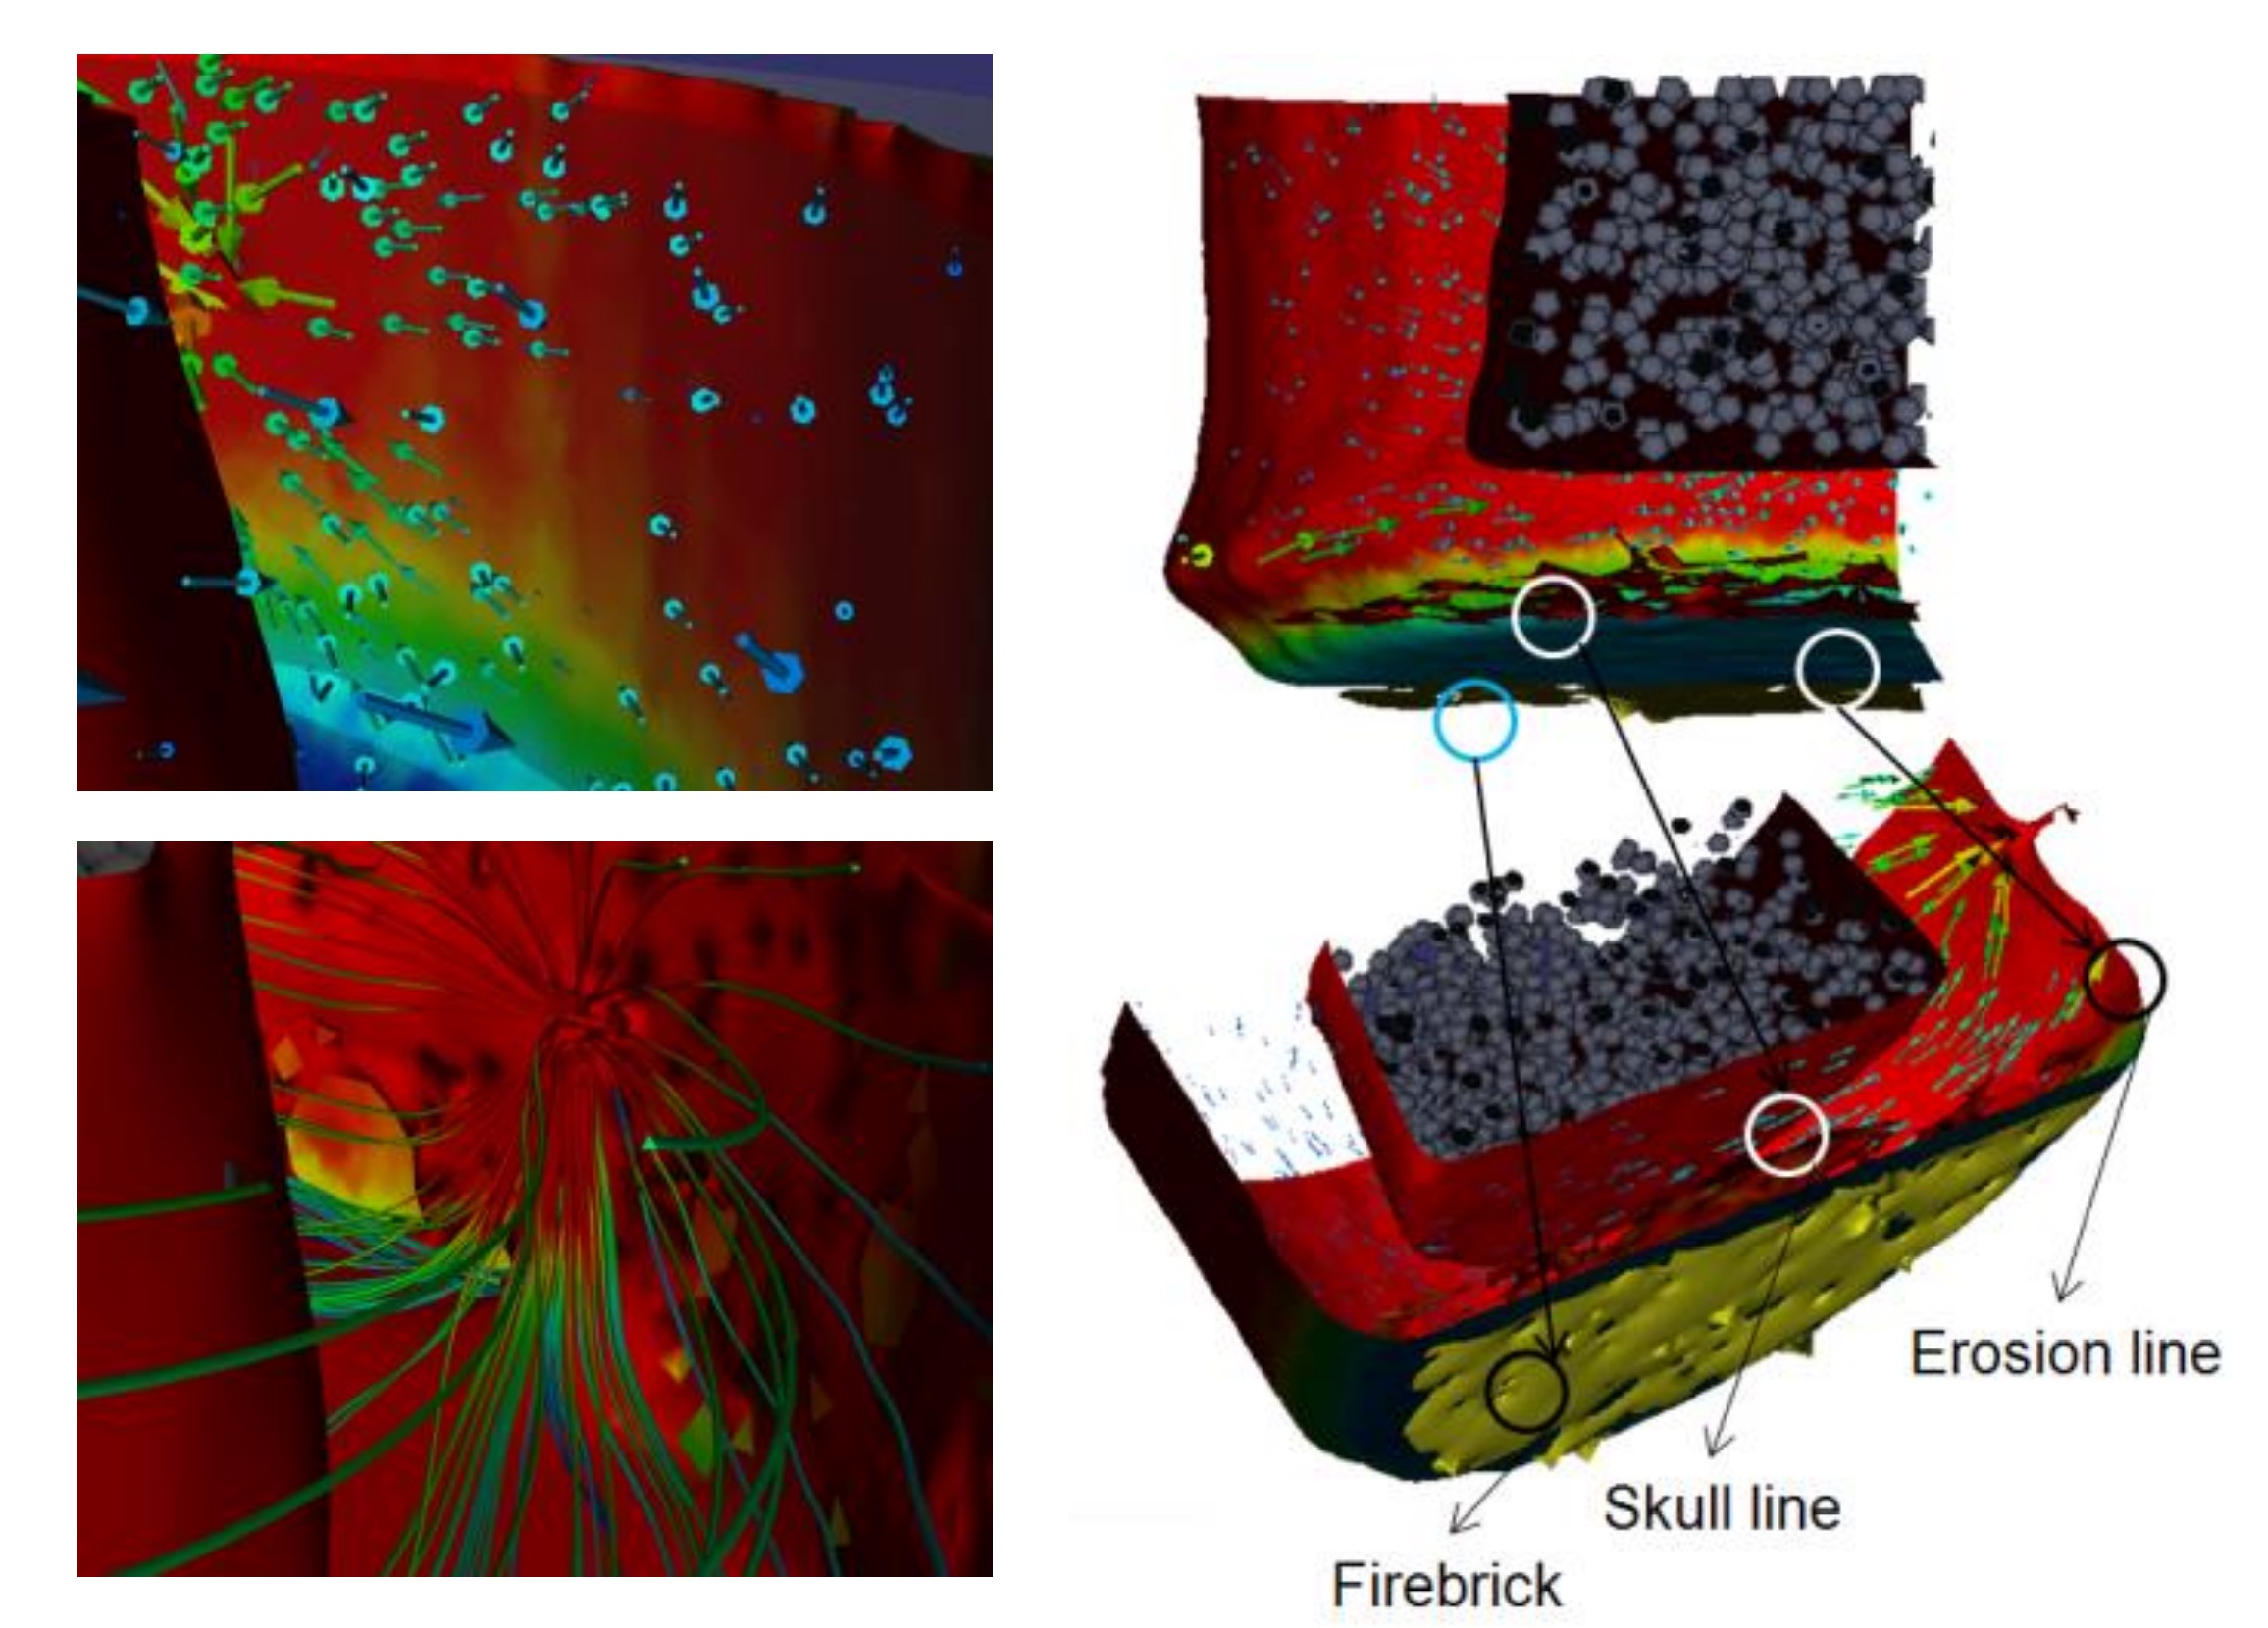
\includegraphics[width=.8\textwidth,angle=0]{figures/blast-furnace-erosion-vr.jpg}
	\caption{3D CFD simulácia a vizualizácia vnútra ("srdca") vysokej pece.}
\end{figure}

Pri numerických simuláciách procesov prúdenia tekutín v kyslíkovom konvertore nie je možné modelovať dostatočne presne všetky fyzikálne javy z dôvodu komplexnosti viacfázových procesov. 

\subsection{Stlačiteľnosť tekutín}

Stlačiteľnosť tekutiny môžeme definovať ako zmenšenie jej objemu v dôsledku vonkajších tlakov na ňu pôsobiacich. Naopak stlačiteľná tekutina zníži svoj objem v prítomnosti vonkajšieho tlaku. Kvantitatívne meranie stlačiteľnosti môžeme popísať ako relatívnu zmenu objemu kvapaliny v reakcii na zmenu tlaku.

Kľúčový rozdiel medzi stlačiteľnými a nestlačiteľnými tekutinami je v tom, že stlačiteľné tekutiny sa vyskytujú v reálnom prostredí, zatiaľ čo nestlačiteľné tekutiny, nazývané aj ideálne tekutiny, sú koncepciou vyvinutou na uľahčenie výpočtu.

Matematicky môžeme stlačiteľnosť $\gamma$ definovať ako

\begin{equation}
	\gamma = \frac{-1}{V} \frac{\partial V}{\partial p}
\end{equation}

kde $V$ je objem tekutiny pred stlačením, $\partial V$ je zmena objemu po sltačení a $\partial p$ je zmena tlaku.

\subsection{Modelovanie turbulencie}

Turbulencia je na prvý pohľad chaotické správanie sa mnohých tekutín. V reálnom živote sú bežné turbulentné toky, medzi ktoré patria napríklad tok krvi kardiovaskulárnym systémom, prúdenie vzduchu okolo krídla lietadla alebo prechod vesmírnych vozidiel atmosférou pri ich návrate na Zem. Napriek desaťročiam výskumu neexistuje analytická teória na predpovedanie vývoja týchto turbulentných tokov. CFD simulácie využívajú modely turbulencie pre predikovanie ich tvorby a evolúcie v simuláciách. Najviac sa používajú dve metódy modelovania turbulencie: simulácia veľkých vírov a Reynoldsovo priemerovanie Navier-Stokesových rovníc.

\begin{figure}[!ht]
	\centering
	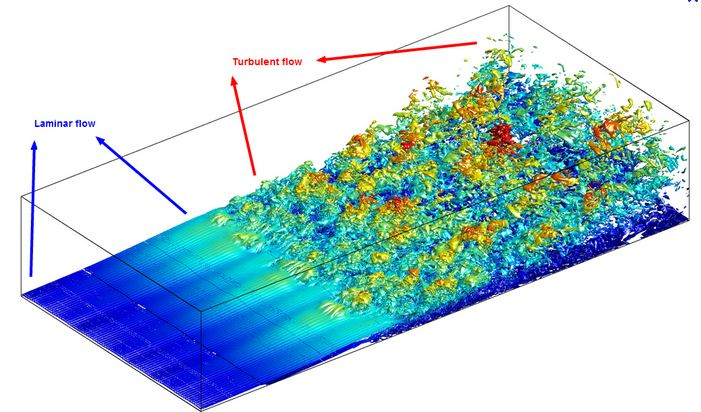
\includegraphics[width=.8\textwidth,angle=0]{figures/turb.jpg}
	\caption{Vizualizácia simulovanej evolúcie turbulentného prúdenia \citep{Vagabond2012}.}
\end{figure}

\section{Navier-Stokesova rovnica}

Navier-Stokesova (NS) rovnica je základným matematickým aparátom na popis prúdenia tekutiny. V praxi má široké využitie, ako napríklad modelovanie minimalizácie odporu vzduchu karosérie áut, návrhu vodných turbín, toku krvi v tele, predpovede počasia a iné. Jej zápis je nasledovný:

\begin{equation}
\frac{\partial \vec{u}}{\partial t} + \vec{u} \cdot \nabla \vec{u} = - \frac{1}{\varrho} \nabla p + \nu \nabla^2 \vec{u} + \vec{g}.
\end{equation}

V praxi sa ňou modeluje hlavne prúdenie nestlačiteľnej (ideálnej) newtonovskej tekutiny, ktorej základná vlastnosť je, že deformácia je priamo úmerná napätiu a jej viskozita je nemenná. Modelovanie stlačiteľnej tekutiny je z hľadiska výpočtového výkonu náročnejšie, čoho dôsledkom je utilizácia vysoko výkonných počítačov a vývoj algoritmov na využitie paralelnej architektúry grafických procesných jednotiek v grafických kartách.

Keďže pri modelovaní systému toku tekutín Navier-Stokesovou rovnicou sa pohybujeme v obore mechaniky tekutín a mechaniky spojitého prostredia (mechanika kontinua), nesmieme zabudnúť na zákon zachovania hmotnosti. Ten popisuje rovnica kontinuity, ktorá v prípade nestlačiteľnej tekutiny nadobúda tvar

\begin{equation}
\frac{\partial \varrho}{\partial t} + \nabla \cdot (\varrho \vec{u}) = 0, 
\end{equation}

kde $\varrho$  je hustota, $t$ je čas, $\nabla \cdot$ je divergencia a $\vec{u}$ je vektorové pole rýchlosti prúdenia.

Pri nestlačiteľnej tekutine zostáva hustota pozdĺž toku v priebehu času konštantná (teda nemenná)

\begin{equation}
\frac{\partial \varrho}{\partial t} = 0, 
\end{equation}

z čoho vyplýva, že divergencia vektorového poľa rýchlosti prúdenia je nulová

\begin{equation}
\nabla \cdot \vec{u} = 0.
\end{equation}

Vo všeobecnosti sú NS rovnice v realite nelineárne parciálne diferenciálne rovnice. Tieto nelinearity sú zodpovedné za turbulencie, ktoré vznikajú pri prúdení tekutín a ktoré tieto rovnice modelujú. Dôvodom vzniku nelinearít je konvekčné zrýchlenie, teda zrýchlenie šírenia tepla prúdením. 

Riešenie NS rovníc pre turbulentné prúdenie tekutiny je extrémne obtiažne, keďže pre dosiahnutie stabilného riešenia je potrebná veľmi detailná sieť. NS rovnice predpokladajú, že skúmaná tekutina je kontinuum (je nekonečne deliteľná a nie je zložená z častíc, ako sú atómy alebo molekuly). Pre modelovanie turbulencie je ale v niektorých prípadoch výhodnejšie využiť alternatívne matematické metódy a iné princípy modelovania (prípadne tieto postupy nejakým spôsobom kombinovať). Vhodnou náhradou sú metódy vychádzajúce z modelovania javov Boltzmannovou rovnicou, akou je napríklad metóda lattice Boltzmann. Táto metóda modeluje prúdenie tekutiny distribučnou funkciou popisujúcou lokálne správanie sa súboru častíc tekutiny v jednotlivých bunkách mriežky, ktorou je model tekutiny obsiahnutý. Vo veľmi malých mierkach alebo v extrémnych podmienkach molekúl tekutiny poskytnú výsledky odlišné od kontinuálnych tekutín modelovaných podľa NS rovníc.

Zaujímavosťou je, že aj napriek praktickému využitiu, zatiaľ neexistuje dôkaz o tom, či riešenia NSR vždy existujú v troch dimenziách, a ak áno, tak či sú na celom intervale nekonečne diferencovateľná. Na tento problém Clayov inštitút vypísal odmenu 1 milión dolárov.

\subsection{Priama numerická simulácia}

Priama numerická simulácia (DNS - Direct Numerical Simulation) je využívaná v odvetví CFD pri riešení NS rovníc priamym spôsobom, bez využitia matematických modelov pre turbulenciu. Numerické riešenie NS rovníc pre turbulentné prúdenie je ale príliš zložité a v súčasnej dobe neexistujú výpočtové prostriedky či algoritmus, ktorý by zabezpečil dostatočne presné riešenie v reálnom čase. V turbulentnom prúdení môžeme pozorovať javy na výrazne rozdielnych úrovniach. Problémom je však diskretizácia: keďže diskretizujeme priestor na oblasti s veľkosťou $\delta x$ (vzdialenosť diskretizačných bodov), nie je možné simulovať víry, ktoré sú menšie ako táto oblasť. Ak by sme chceli nasimulovať úplné detaily, potrebovali by sme použiť veľmi vysoké rozlíšenie, pričom súčasné výpočtové prostriedky na to nepostačujú.

\section{Metóda lattice Boltzmann}

Metóda lattice Boltzmann (LBM) je relatívne nová metóda v oblasti CFD analýzy. V posledných niekoľkých desaťročiach sa dosiahol veľký pokrok v jej vývoji. Je založená na pohybe súboru častíc a v porovnaní s konvenčnými metódami založenými na kontinue dokáže detailnejšie modelovať komplexné geometrie a hlavne významne zredukovať čas riešenia simulácie z dôvodu vysokej paralelizácie výpočtu. LBM sa postupom času vyvinula na všestrannú a výkonnú výpočtovú metodológiu pre základné výskumné aj inžinierske aplikácie. V súčasnosti si nachádza svoje využitie v širokej škále odborov vrátane fyziky, chémie materiálov, biomedicíny a rôznych odborov strojárstva.

\begin{figure}[!ht]
	\centering
	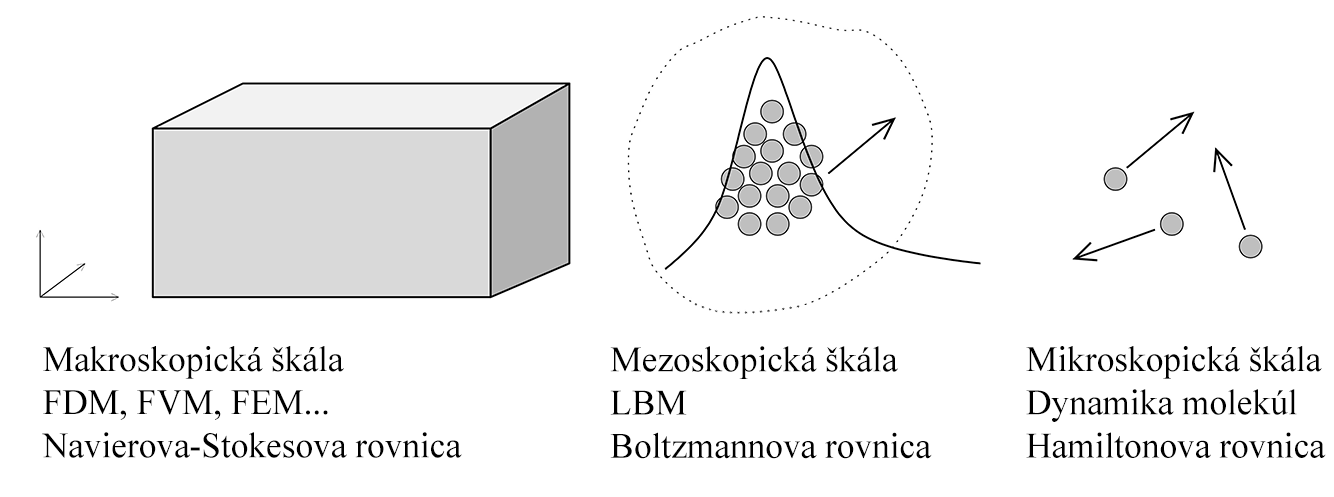
\includegraphics[width=1\textwidth,angle=0]{figures/different-scales.png}
	\caption{Techniky simulácie v rôznych škálach \citep{Mele2013}.}
	\label{o:scales}
\end{figure}

Základnou myšlienkou LBM je zostrojiť zjednodušené kinetické modely na mezoskopickej mierke, ktoré premosťujú mikroskopické a makroskopické mierky a začleňujú základnú fyziku mikroskopických procesov tak, aby potom výsledné makroskopické vlastnosti po určitom spriemerovaní dodržiavali požadované makroskopické rovnice. Tekutina je pri tomto prístupe rozdelená na diskrétne polia mriežkou. Dôvod, prečo je možné použiť zjednodušené kinetické modely je ten, že makroskopická dynamika tekutiny je výsledkom kolektívneho správania sa mnohých mikroskopických častíc v systéme \citep{Mele2013}, takže pri pohľade na problémy s veľkosťou a časom niekoľko rádov nad veľkosťou molekúl je možné považovať tekutinu za kontinuálne médium (obr. \ref{o:scales}) a ignorovať jej diskrétnu povahu bez významných chýb vo výpočtoch. Vlastnosti súboru mikroskopických častíc popisuje distribučná funkcia, ktorá hrá pri metóde lattice Boltzmann dôležitú úlohu.

\begin{figure}[!ht]
	\centering
	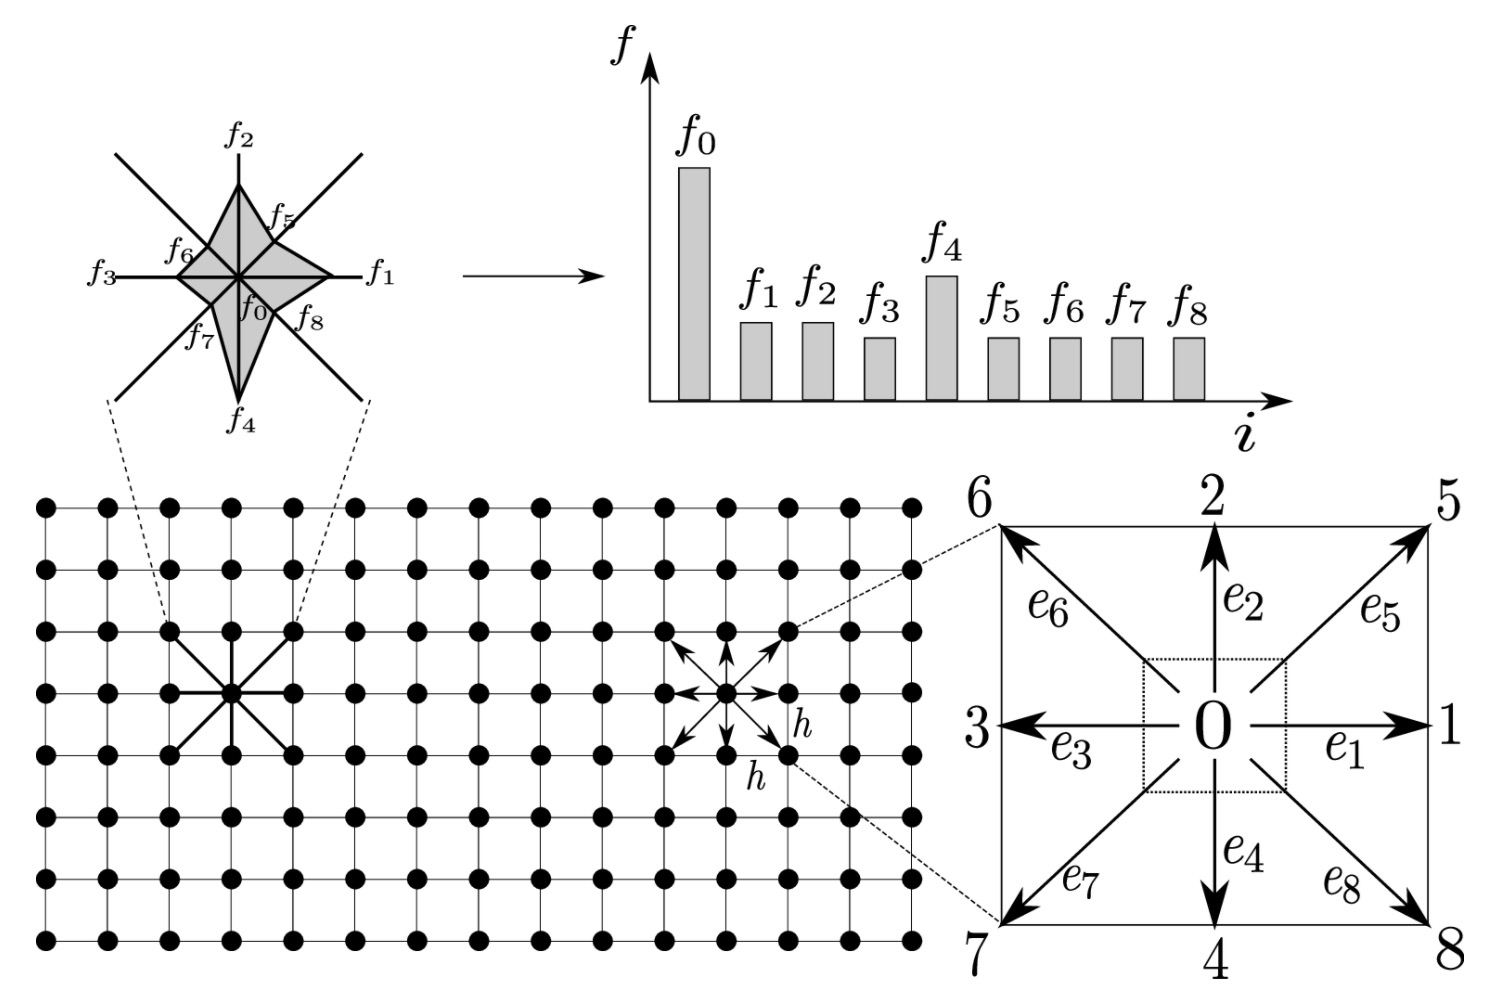
\includegraphics[width=.8\textwidth,angle=0]{figures/lbm-grid.jpg}
	\caption{Mriežková štruktúra LBM \citep{Soga2020}.}
\end{figure}

LBM je založená na riešení Boltzmannovej rovnice popisujúcej štatistické rozdelenie jednej častice v tekutine v šesť-dimenzionálnom fázovom priestore. LBM popisuje vývoj distribučnej funkcie $f = (\vec{x}, \vec{e}, t)$ v čase. Tá sa môže meniť v dôsledku vzájomných kolízií častíc, ktoré pri nárazoch menia svoju hybnosť a energiu, a to v dôsledku vlastného pohybu častíc alebo vplyvom externých síl \citep{HEIDLER2011thesis}. Častica môže ostať v pôvodnej bunke mriežky alebo môže byť odrazená do jednej zo susedných buniek. Konfigurácia častíc pri každom časovom kroku sa vyvíja v dvoch postupných čiastkových krokoch:

\begin{itemize}
	\item Častice skočia z jedného mriežkového uzla do nasledujúceho podľa svojej (diskrétnej) rýchlosti. Toto je propagačná fáza (streaming).
	\item Potom sa častice zrazia a získajú novú rýchlosť. Toto je fáza kolízie (collision).
\end{itemize}

Pravidlá upravujúce zrážky sú navrhnuté tak, aby priemerný čas vyhovoval zachovaniu hmotnosti a hybnosti.

Distribučná funkcia závisí od vektora polohy častíc $\vec{x}$, vektora rýchlosti častíc $\vec{e}$ a času $t$. $f(\vec{x}, \vec{e}, t)$ reprezentuje počet častíc s hmotnosťou $m$ polohovo rozmiestnených v čase $t$ medzi $\vec{x} + d\vec{x}$ pohybujúcich sa rýchlosťou $\vec{e} + d\vec{e}$, ktorých smer a rýchlosť sa zmení v čase $t + dt$ v dôsledku pôsobenia externej sily $F$ (táto zmena je vyjadrená vzťahom $\vec{e} + \frac{F}{m}dt$).

\begin{figure}[!ht]
	\centering
	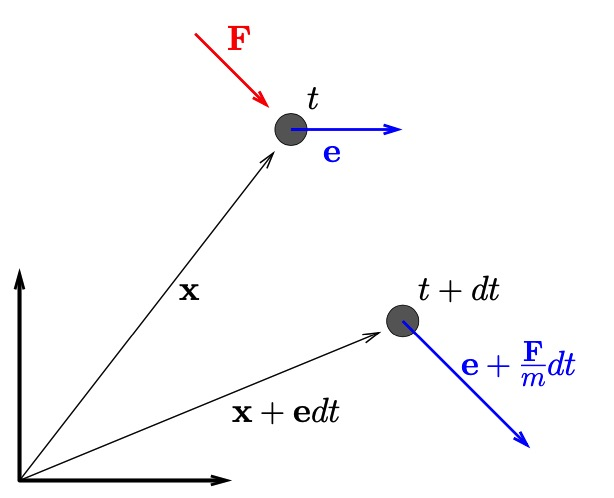
\includegraphics[width=.4\textwidth,angle=0]{figures/collision-vector.jpg}
	\caption{Pozičný vektor $\vec{x}$ a rýchlostný vektor $\vec{e}$ pred a po aplikovaní externej sily $F$ \citep{Mele2013}.}
\end{figure}

Ak nedôjde ku kolízii častíc, počet častíc pred a po aplikovaní externej sily $F$ ostáva nezmenený:

\begin{equation}
f(\vec{x} + \vec{e}dt, \vec{e} + \frac{\vec{F}}{m}dt, t + dt)d\vec{x}d\vec{e} = f(\vec{x},\vec{e},t)d\vec{x}d\vec{e}.
\end{equation}

V prípade kolízie dôjde k zmene distribúcie častíc. Zmena distribučnej funkcie je potom vyjadrená kolíznym operátorom $\Omega$. Zapísať túto zmenu môžeme nasledovne:

\begin{equation}
f(\vec{x} + \vec{e}dt, \vec{e} + \frac{\vec{F}}{m}dt, t + dt)d\vec{x}d\vec{e} - f(\vec{x},\vec{e},t)d\vec{x}d\vec{e} = \Omega(f)d\vec{x}d\vec{e}dt.
\end{equation}

Rovnicu po úprave môžeme zapísať ako

\begin{equation}
\frac{Df}{dt} = \Omega(f)
\end{equation}

pri $dt$ blížiace sa 0. Z tejto rovnice vyplýva, že celková rýchlosť zmeny distribučnej rovnice sa rovná miere kolízie. 

Pri LBM je priestor diskretizovaný takou formou, aby bol konzistentný s kinetickou rovnicou. Kinetická forma distribučnej funkcie je potom definovaná ako

\begin{equation}
f_k(\vec{x} + \vec{e}_k \Delta t,  t + \Delta t) = f_k(\vec{x},t) + \Omega_k(f(\vec{x},t)), \quad k = 1, ...M,
\end{equation}

kde $\Delta t$ je časový inkrement a $f_k$ je distribúcia rýchlosti častice v smere $k$. Pre zjednodušenie Boltzmannovej rovnice bez toho, aby sa narušila fyzika systému, zaviedli \cite{bhatnagar1954} kolízny operátor BGK:

\begin{equation}
\Omega_k = - \frac{1}{\tau}(f_k-f_k^{EQ})
\end{equation}

kde $\tau$ je relaxácia častíc pri vzájomných zrážkach smerom k lokálnej rovnováhe (relaxácia úzko súvisí s viskozitou tekutiny), $f_k^{EQ}$ je distribučná funkcia rovnováhy (equilibrium).

Pravú stranu Boltzmannovej rovnice môžeme upraviť nasledovne:

\begin{equation}
\frac{\partial f}{\partial t} + \vec{e} \cdot \nabla f = - \frac{1}{\tau}\left(f-f^{EQ}\right).
\end{equation}

Pre špecifický smer v mriežke ma funkcia tvar

\begin{equation}
\frac{\partial f_k}{\partial t} + \vec{e_k} \cdot \nabla f_k = - \frac{1}{\tau} \left(f_k-f_k^{EQ} \right)
\end{equation}

a táto rovnica následne pri CFD simuláciách nahrádza Navier-Stokesove rovnice. Úplne diskretizovaná rovnica s časovým krokom $\Delta t$ a priestorovou zmenou \\ $\Delta x_k=\vec{e_k}\Delta t$ je

\begin{equation}
f_k(\vec{x}_k + \vec{e}_k \Delta t,  t + \Delta t) = f_k(\vec{x}_k,t) - \frac{\Delta t}{\tau} \left(f_k-f_k^{EQ} \right).
\end{equation}

Pre deväť-rýchlostný model je definovaný rýchlostný vektor nasledovne:

\begin{equation}
\vec{e} = \left\{
\begin{array}{ll}
(0,0), & \quad k = 0, \\
e\left[cos \frac{(k-1)\pi}{4}, sin \frac{(k-1)\pi}{4}\right], & \quad k = 1,3,5,7 \\
\sqrt{2e}\left[cos \frac{(k-1)\pi}{4}, sin \frac{(k-1)\pi}{4}\right], & \quad k = 2,4,6,8, \\
\end{array}
\right.
\end{equation}

\begin{figure}[!ht]
	\centering
	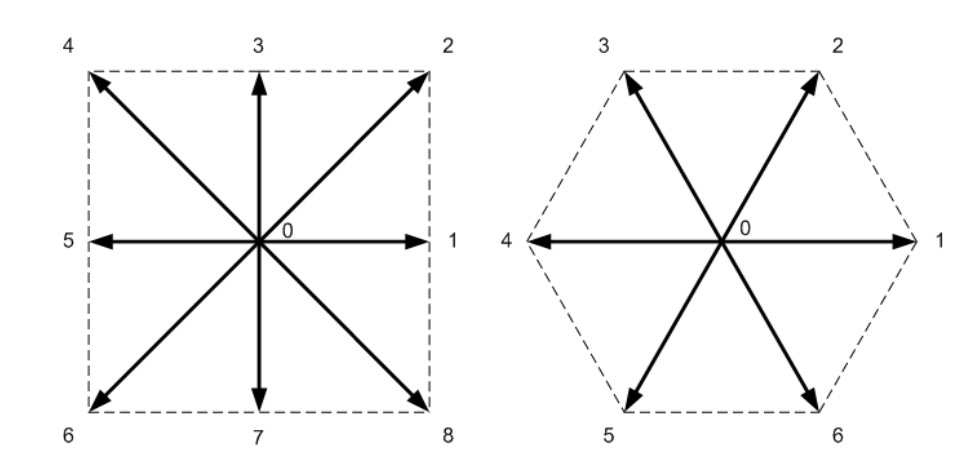
\includegraphics[width=.54\textwidth,angle=0]{figures/lbm-lattices.jpg}
	\caption{Grafické znázornenie 2D modelov LBM. Deväť-rýchlostný (D2Q9) model naľavo a sedem-rýchlostný (D2Q7) model napravo.}
\end{figure}


\section{Programy pre CFD simulácie}

V tejto kapitole veľmi stručne uvediem niektoré programy, ktoré sa v súčasnosti využívajú pre tvorbu CFD simulácií a vizualizácií.

\subsection{Matlab}

Matlab obsahuje niekoľko toolboxov pre CFD analýzu. Spomeniem dve najpoužívanejšie (podľa počtu stiahnutí): FEATool Multiphysics a CFDTool.

FEATool Multiphysics je simulačný nástroj pre CFD analýzu, modelovanie prenosu tepla, štrukturálnych zmien súčiastok, elektromagnetických javov a iné. Poskytuje intuitívne grafické rozhranie, ponúka nástroje pre úpravy geometrie CAD modelov, generáciu mriežky v rámci skúmanej oblasti a taktiež výber z viacerých integrovaných solverov.

CFDTool ponúka podobnú funkcionalitu ako FEATool, no zameriava sa hlavne na modelovanie toku tekutín a prenos tepla

Implementácia LBM je v Matlabe možná v pár riadkoch kódu bez použitia externých knižníc. Niekoľko ukážkových implementácií je dostupných na webe projektu Palabos od Ženevskej univerzity \citep{Palabos2020}.

\subsection{Ansys Fluid}

Softvér Ansys Fluent poskytuje široké možnosti fyzikálneho modelovania potrebné na modelovanie toku, turbulencie, prenosu tepla a chemických reakcií pre priemyselné aplikácie, akými sú prúdenie vzduchu cez krídlo lietadla, spaľovanie v peci, tvorba bublín a bublinových stĺpcov v tekutinách, prietok krvi, optimalizácia dizajnu polovodičov alebo návrh čističky odpadových vôd. Ansys Fluent má veľmi dlhú históriu a počas niekoľkých posledných dekád sa stále umiestňuje na prvých priečkach využiteľnosti medzi firmami využívajúcimi CFD simulácie. Je to z dôvodu nespočetného množstva predpripravených modelov a jednoduchosti užívateľského prostredia.

\subsection{SimScale}

Platforma SimScale ponúka v rámci čiastkových produktov mnohé funkcionality ako ostatné simulačné programy, no táto firma stavila na využitie cloudových technológií. Práca s programom prebieha cez webové rozhranie, kde užívateľ nastavuje a spúšťa simulácie a taktiež sa priamo vo webovom prehliadači zobrazuje 2D alebo 3D vizualizácia simulovaného modelu. Výpočty prebiehajú na serveroch prevádzkovaných alebo prenajímaných firmou SimScale, využívajúce možnosti masívnej paralelizácie pomocou grafických kariet.

\begin{figure}[!ht]
	\centering
	\subfloat[Simulácia toku vetra okolo modelu niekoľkých výškových budov so zložitou geometriou.]{{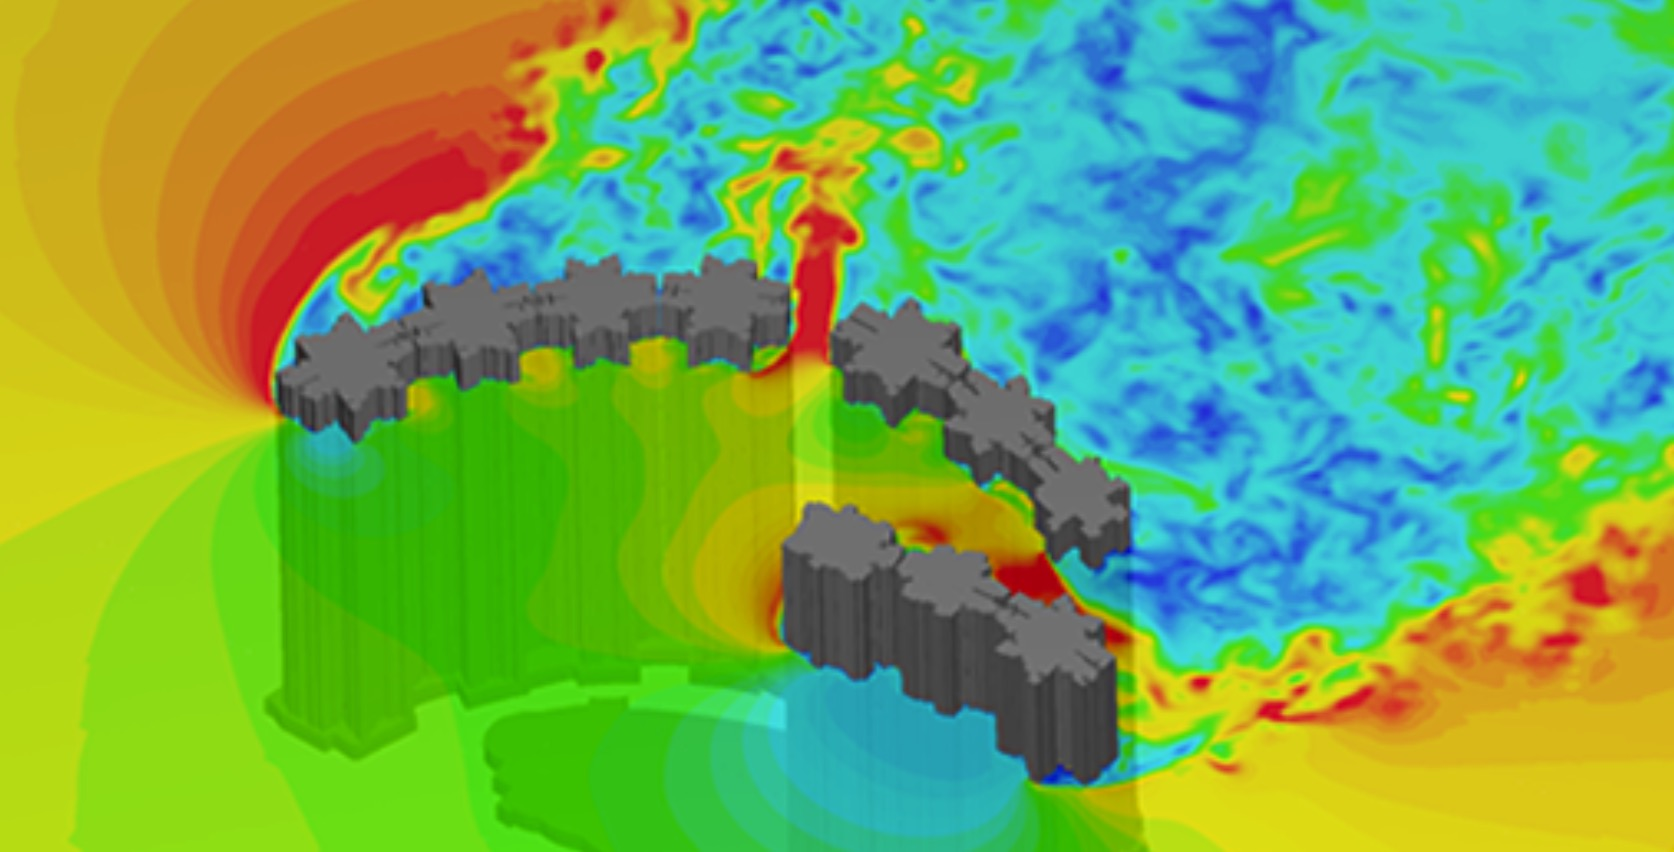
\includegraphics[width=7.1cm]{figures/simscale-cfd.jpg} }}%
	\qquad
	\subfloat[CFD simulácia viacfázovej tekutiny.]{{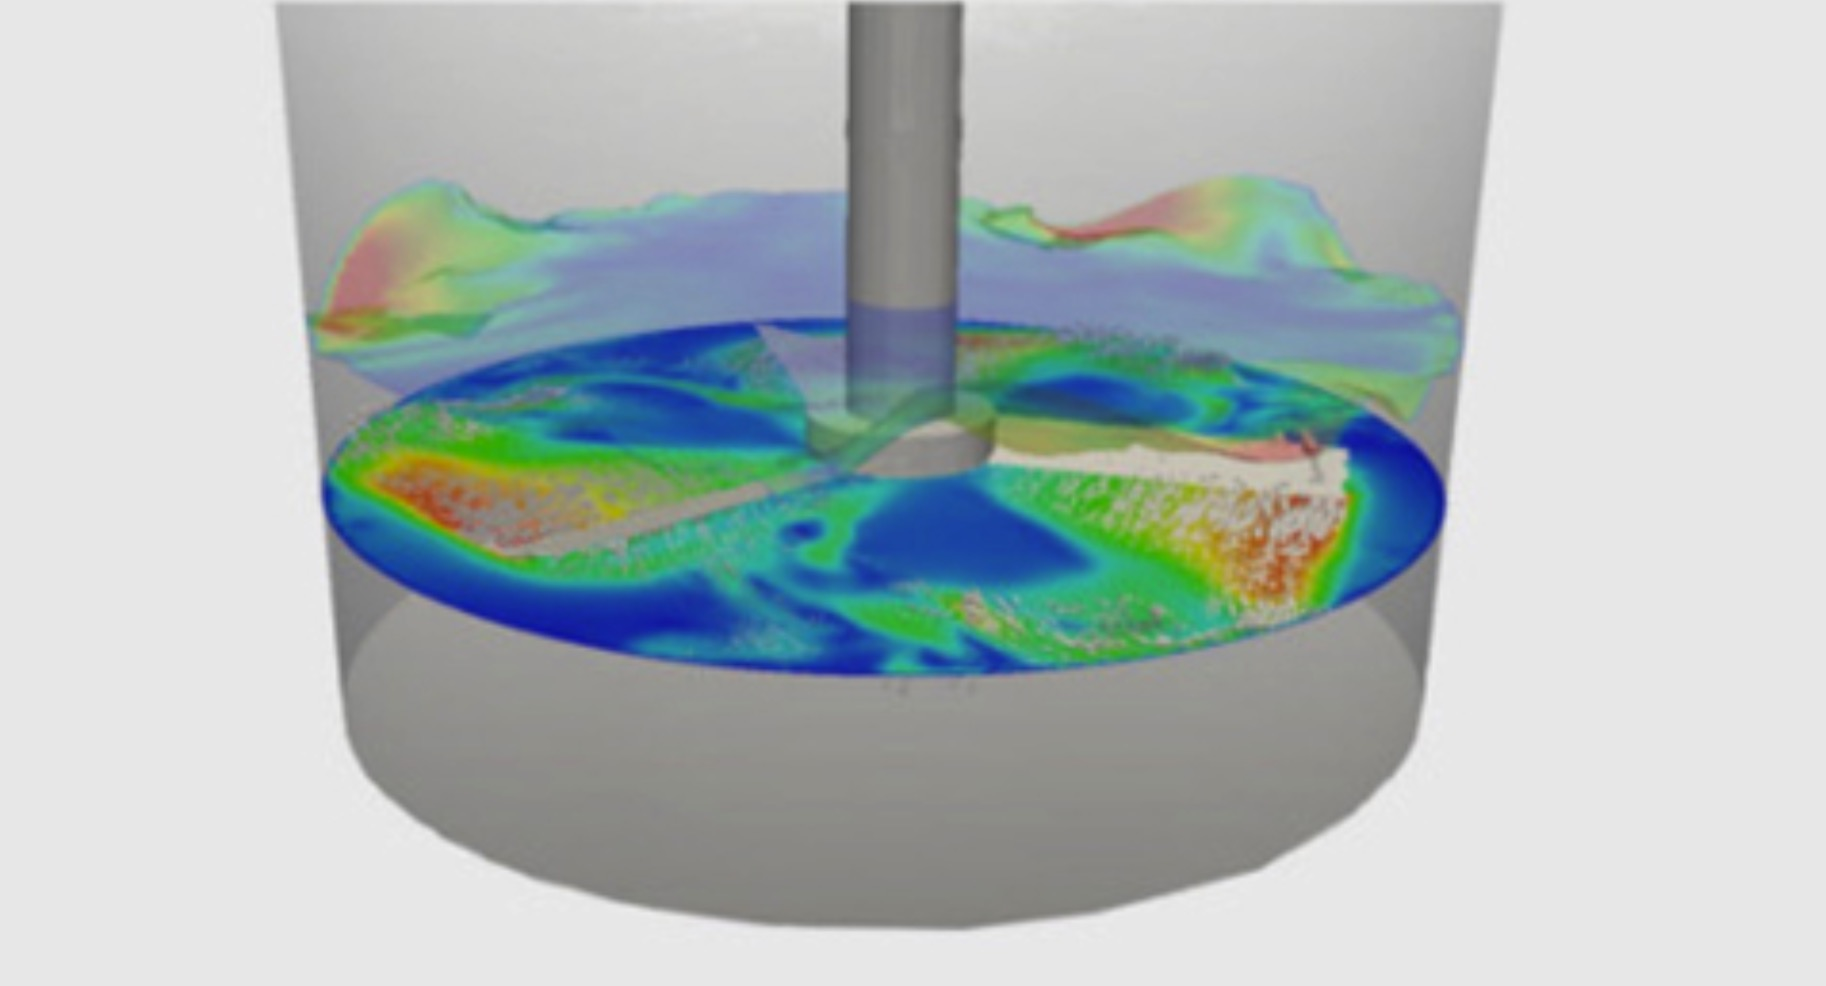
\includegraphics[width=6.7cm]{figures/simscale-multiphase.jpg} }}
	\caption{Vizualizácie CFD simulácií v prostredí SimScale.}
\end{figure}

\subsection{OpenFOAM}

OpenFOAM je súbor nástrojov s voľne prístupným zdrojovým kódom na riešenie zložitých problémov s výpočtovou dynamikou tekutín. Obsahuje širokú škálu fyzikálnych modelov (vrátane turbulencie, úprav stien hraničných podmienok - geometrie, termodynamiky a hromadnej dopravy), numerických metód a nástrojov na predbežné a následné spracovanie.

\subsection{OpenLB}

OpenLB je balík C++ modulov pre implementáciu lattice Boltzmann simulácií určený predovšetkým ako programová podpora pre výskumníkov a technikov, ktorí simulujú toky tekutín pomocou LBM. Podporuje komplexné dátové štruktúry, pomocou ktorých je možné simulovať zložité geometrie. Diskretizovať geometrie (meshing alebo voxelizácia) z dopredu pripravených 3D modelov a nastaviť okrajové podmienky je možné automaticky - automatickým predspracovaním (aj komplexného) 3D modelu. Paralelizácia v implementovaných algoritmoch je riešená využitím knižnice OpenMP, z čoho môžu benefitovať výkonné multiprocesorové viacjadrové počítače (v architektúrach využívajúcich zdieľanú pamäť). Pri distribuovaných počítačových systémoch, na ktorých by sme chceli simulovať modely na báze LBM pomocou OpenLB majú paralelné algoritmy v tomto balíku implementované rozhranie na posielanie a prijímanie správ medzi jednotlivými procesmi (MPI - Message-Passing Interface)

\section{Záver}

Simulácie sú neoddeliteľnou súčasťou počítačom podporovaného inžinierstva ako aj vedeckého skúmania fyzikálnych javov. Výsledkom simulácie je približné, no dostatočne presné riešenie modelovanej úlohy. Modelovanie na základe matematických metód prešlo dekádami vývoja a vylepšovanie metód pokračuje neustále naďalej. V oblasti počítačovej dynamiky tekutín (CFD) v posledných rokoch významne vzrástol záujem o skúmanie nových metód matematického a fyzikálneho modelovania. Jednou z týchto metód je metóda lattice Boltzmann, ktorá ponúka výrazné skrátenie konvergencie výpočtu a vyššiu mieru presnosti. Vďaka rozdeleniu riešeného problému správania sa tekutiny do diskrétnych buniek tvoriacich mriežku a modelovaniu pohybu ako súboru lokálnych častíc, je simuláciu možné prevádzať paralelnými výpočtami. Signifikantné zrýchlenia času simulácie sa dosahuje využitím architektúry grafických procesných jednotiek (GPU). CFD simulácie fyzikálnych javov v kyslíkovom konvertore, využívajúce metódu lattice Boltzmann, budú súčasťou mojej dizertačnej práce.

%
%%
\Urlmuskip=0mu plus 1mu\relax
\bibliographystyle{spbasic}
\bibliography{refs/control,refs/mathematics,refs/modeling,refs/cfd,refs/lbm,refs/gpu,refs/interaction,refs/interfaces,refs/hci,refs/design,refs/ml,refs/visualization,refs/programming,refs/simulation,refs/ar,refs/vr,refs/online}

%

\end{document}
%%